\begin{tframe}{Validation}

The set of faces used in the training of the models might not be completely clean:

\begin{itemize}
\item If an image contains two faces, each of them will have the same ranking; thus, if the ranking is high, they will both be used in the training phase but only one of them will correctly represent the identity.
\item The same can be said about false positive detection.
\end{itemize}

\vspace{0.1in}

Since it is not possible to resolve these problems in the previous steps, we have classification models that have been obtained with training sets containing errors.

\begin{figure}[h]
\centering
\hspace*{\fill}
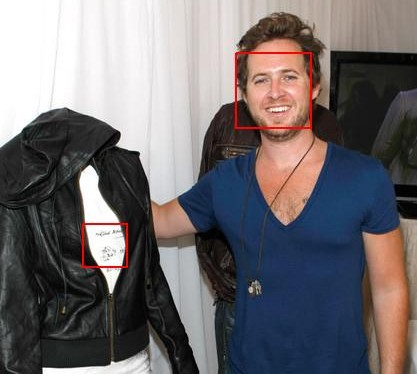
\includegraphics[width=0.30\textwidth]{images/image1a.jpg}
\hspace*{\fill}
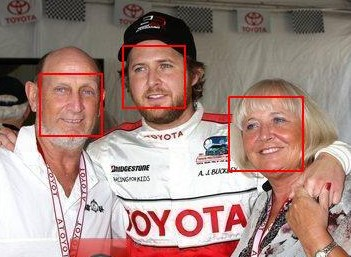
\includegraphics[width=0.30\textwidth]{images/image2a.jpg}
\hspace*{\fill}
\end{figure}

\end{tframe}


\begin{tframe}{Validation}

A \textbf{web application} for \textbf{visual validation} has been created for this purpose, thanks to which are shown to a \textbf{user} the images associated to each identity along with the results of the classification.

\vspace{0.1in}

A \textbf{user} can interact with the web application, by browsing each identity and the images that are shown in a gallery; the user can also double click an image to \textbf{correct} the results of the classification. A user can also decide to completely remove an identity from the dataset.

\begin{figure}[h]
\begin{center}
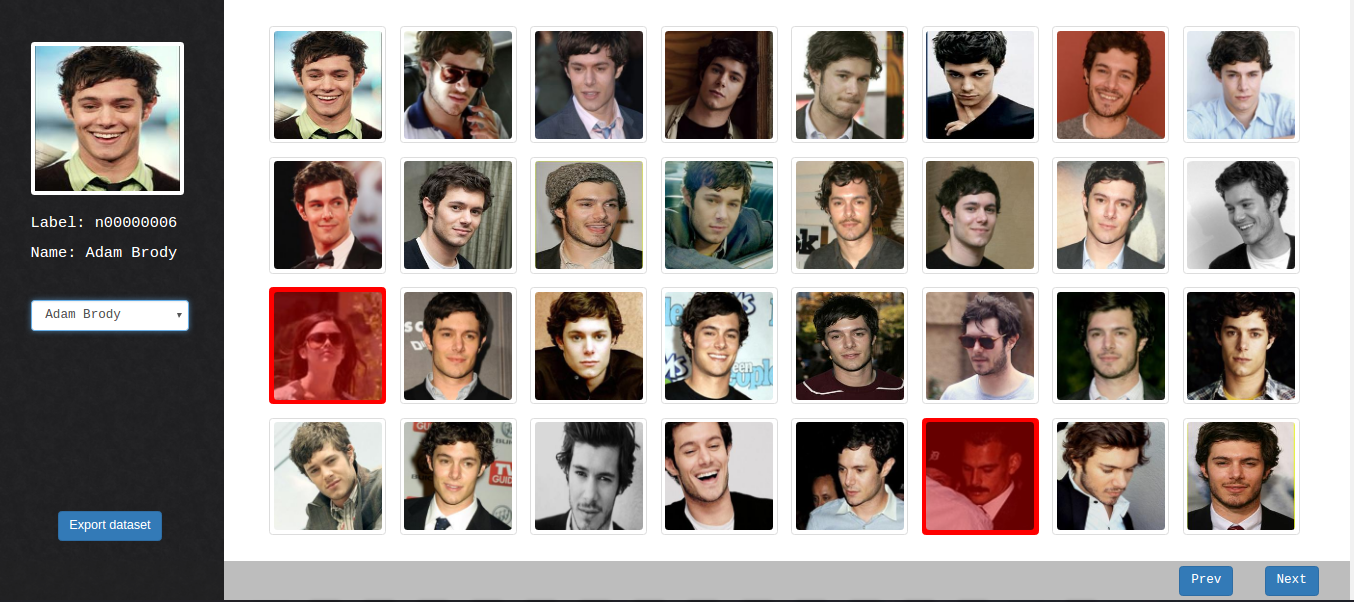
\includegraphics[width=0.75\textwidth]{images/image5.png}
\end{center}
\end{figure}

\end{tframe}